\chapter{Integrali multipli}
Il capitolo che segue espone la teoria dell'integrazione di funzioni di $n$ variabili. La trattazione affronterà in prima istanza il tema della misura secondo Peano-Jordan. Dopodiché si passerà al caso degli integrali doppi con funzioni di $n=2$ variabili. Verranno mostrati in seguito i metodi di integrazione di funzioni in $n=3$ variabili, per concludere con gli integrali impropri.
\section{Misura di Peano-Jordan}
\begin{definition} \label{Def: Rettangolo}
Sia $I=\left[a_1, b_1\right) \times \left[a_2, b_2 \right) \times \dots \times \left[a_n, b_n \right)$ con $a_i < b_i$. Allora, tale intervallo è definito \textbf{rettangolo} superiormente semiaperto di $\mathbb{R}^n$.\\
Inoltre, si definisce \textbf{misura elementare} di $I$ il volume di tale rettangolo, cioè:
\begin{equation}
    m(I)=\left(b_1-a_1\right)\left(b_2-a_2\right)\dots\left(b_n-a_n\right)
\end{equation}
\end{definition}
\begin{oss}
    Se $I$ è vuoto, allora si pone per convenzione $m(I)=0$.
\end{oss}
\begin{oss}
    La scelta di intervalli semiaperti superiormente permette di poter creare partizioni senza problemi di sovrapposizione.
\end{oss}
\begin{definition} \label{Def: Plurirettangolo}
    Si dice \textbf{plurirettangolo} superiormente semiaperto di $\mathbb{R}^n$ un insieme $P$ dato dall'unione finita di rettangoli superiormente semiaperti a 2 a 2 disgiunti, cioè
    \begin{equation}
        P= \bigsqcup_{j=1}^{H \in \mathbb{N}} I_j \qquad I_j \cap I_l = \emptyset\ \text{se}\ j\neq l
    \end{equation}
\end{definition}
\begin{definition} \label{Def: Misura di un plurirettangolo}
Sia $\mathcal{P}= \left\{\text{insieme dei plurirettangoli}\right\}$. Allora si dice \textbf{misura di un plurirettangolo} $P=\bigsqcup\limits_{j=1}^{H} \in \mathcal{P}$ la quantità
\begin{equation}
    m(P)= \sum_{j=1}^{H}{m(I_j)}
\end{equation}
\end{definition}
\begin{oss}
    Si osservi che la scelta di una partizione per $P$ è ininfluente ai fini del calcolo della misura di un plurirettangolo.
\end{oss}
Queste definizioni, permettono di sviluppare una funzione $m: \mathcal{P} \to \mathbb{R}^+$ che goda delle seguenti proprietà $ \forall\ P_1, P_2\in \mathcal{P}$:
\begin{itemize}
    \item $m$ è \textbf{subadditiva}: $m(P_1 \cup P_2) \leq m(P_1)+m(P_2)$
    \item $m$ è \textbf{additiva}: $m(P_1 \cup P_2)=m(P_1)+m(P_2)$ se $P_1 \cap P_2 = \emptyset$
    \item $m$ è \textbf{crescente}: se $P_1 \subseteq P_2$ allora $m(P_1) \leq m(P_2)$
\end{itemize}
\begin{definition} \label{Def: Misura interna, misura esterna}
Sia $E \subseteq \mathbb{R}^n$. Allora, si definisce \textbf{misura esterna} di E la quantità 
\begin{equation}
    \overline{m}(E) := \inf\left\{m(P) \mid P \in \mathcal{P}, E \subseteq \mathcal{P} \right\}
\end{equation}
Analogamente, si definisce \textbf{misura interna} di E la quantità
\begin{equation}
    \underline{m}(E) := \sup\left\{m(P) \mid P \in \mathcal{P}, E \subseteq P\right\}
\end{equation}
\end{definition}
\begin{proposition}
    Sia $E \subseteq \mathbb{R}^n$ limitato. Allora $\underline{m}(E) \leq \overline{m}(E)$
\end{proposition}
\begin{definition} \label{Def: Insieme misurabile}
    Si dice che $E \subseteq \mathbb{R}^n$ è \textbf{misurabile} secondo Peano-Jordan se
    \begin{equation}
        \underline{m}(E)=\overline{m}(E)
    \end{equation}
    In tal caso allora
    \begin{equation}
        m(E) := \underline{m}(E)=\overline{m}(E)
    \end{equation}
    e si indica con $\mathcal{M}$ l'\textbf{insieme degli $\mathbf{E}$} limitati e \textbf{misurabili} di $\mathbb{R}^n$
\end{definition}
\begin{oss}
    Una notazione alternativa di $m(E)$ è $m_n(E)$
\end{oss}
\begin{oss}
    Si noti che $\mathcal{M} \subsetneq \mathcal{P}(\mathbb{R}^n)$
\end{oss}
\begin{example}
    A sostegno di quest'ultima osservazione si proponga un insieme non misurabile di $\mathbb{R}^n$
    \begin{equation*}
        \Tilde{E}=\left( \left[0,1\right] \cap \mathbb{Q}^2\right)
    \end{equation*}
    Infatti, volendo coprire di plurirettangoli tale insieme, si ha che:
    \begin{align*}
        &\overline{m}(\Tilde{E})=1=(1-0)\times(1-0)\\
        &\underline{m}(\Tilde{E})=0
    \end{align*}
    Pertanto $\Tilde{E}$ non è misurabile secondo Peano-Jordan.
\end{example}
D'altro canto, si elenchino ora tipi di insiemi che siano Peano-Jordan misurabili.
\begin{example}
    Il caso banale è il plurirettangolo P. Infatti:
    \begin{equation*}
    m(P)=m(\mathring{P})=m(\overline{P})       
    \end{equation*}
\end{example}
\begin{example} \label{Def: Dominio normale}
    Un \textit{dominio semplice}, cioè un dominio compreso tra i grafici di funzioni continue su $\left[a,b\right]$ limitate, è P.J. misurabile.
    
    In $\mathbb{R}^2$ si possono avere domini semplici della forma:
    \begin{equation*}
            D= \left\{ (x, y) \in \mathbb{R}^2 \mid a \leq x \leq b ,\ f(x)\leq y \leq g(x) \right\}\        
    \end{equation*}
    detti \textit{y-semplici} o \textit{normali rispetto all'asse x}. Oppure
    \begin{equation*}
        E= \left\{(x, y) \in \mathbb{R}^2\mid c \leq y \leq d,\ h(y) \leq x \leq l(y)\right\}
    \end{equation*}
    detti \textit{x-semplici} o \textit{normali rispetto all'asse y}.
    \vspace*{6pt}                       
    
    In $\mathbb{R}^3$ esempi di domini semplici possono essere:
    \begin{equation*}
        \mathcal{D}=\left\{(x,y,z) \in \mathbb{R}^3 \mid (x,y) \in D \subseteq \mathbb{R}^2,\ \alpha(x, y) \leq z \leq \beta(x,y) \right\}
    \end{equation*}
    con $D$ normale rispetto ad almeno un asse e detto \textit{z-semplice} o \textit{normale rispetto al piano xy} o, ancora \textit{rappresentabile per fili}. Oppure, 
    \begin{equation*}
        \mathcal{E}=\left\{(x,y,z) \in \mathbb{R}^3 \mid c_1 \leq z \leq c_2,\ (x,y) \in D(z)\subseteq \mathbb{R}^2\right\}
    \end{equation*}
    con $D_z$ dominio normale e detto \textit{xy semplice} o \textit{normale rispetto all'asse $z$} o \textit{rappresentabile per strati}.
\end{example}
    \begin{oss}
        Si possono ottenere altri domini normali di $\mathbb{R}^3$ invertendo gli assi.
    \end{oss}
    \begin{oss}
        Se $D$ è un dominio normale rispetto a $x$, si ha che
        \begin{equation}
            m(D)= \int_a^b(g(x)-f(x))dx
        \end{equation}
        Lo stesso discorso vale poi per domini semplici di $\mathbb{R}^3$. Infatti
        \begin{equation}
            \begin{aligned}
                &m(\mathcal{D})=\iint\limits_D(\beta(x,y)-\alpha(x,y))dxdy\\
                &m(\mathcal{E})=\int_{c_1}^{c_2}(m_z(D_z))dz
            \end{aligned}
        \end{equation}
    \end{oss}
    \subsection{Proprietà della misura di Peano-Jordan}
    Siano $A, B \in \mathcal{M}$. Allora, si può osservare che l'unione, l'intersezione e la differenza di insiemi misurabili è misurabile.
    \begin{equation}
        A \cup B,\ A \cap B,\ A \setminus B \in \mathcal{M}
    \end{equation}
    Rispetto a ciò, per \textbf{subadditività}, la misura dell'unione vale:
    \begin{equation}
        m(A \cup B) = m(A)+ m(B)- m(A \cap B)
    \end{equation}
    e, in particolare, se l'intersezione dei due insiemi è vuota, vale l'\textbf{additività finita}, cioè:
    \begin{equation}
        m(A \cup B) = m(A)+ m(B)
    \end{equation}
    Per quanto riguarda la misura della differenza dei due insiemi si nota che 
    \begin{equation}
        m(A \setminus B)= m(A)-m(A \cap B)
    \end{equation}
    e, nello specifico, se $B \subseteq A$,
    \begin{equation}
        m(B) \leq m(A)
    \end{equation}
    per \textbf{monotonia}.\\
    Infine $E \subseteq \mathbb{R}^n$ limitato è misurabile se e solo se la sua frontiera $\partial E$ è misurabile ed ha misura nulla.
\section{Introduzione agli integrali multipli}
Si descriva ora il processo di costruzione degli integrali in più variabili tramite l'utilizzo delle somme superiori e inferiori di Riemann.

D'ora in avanti si considerino $A \subseteq \mathbb{R}^n$ aperto con $A \in \mathcal{M}$ e $f:A \to \mathbb{R}$ limitata. Si prenda poi poi $P=\left\{ A_i \right\}_{i=1}^{N}$ una partizione finita di $A$ di insiemi misurabili secondo Peano-Jordan, cioè tale che
    \begin{equation}
    A= \bigsqcup A_i \qquad A_i \in \mathcal{M}\ \forall\ i
    \end{equation}
\begin{definition} \label{Def: Somme di Riemann}
Con le premesse sopra, si dicono \textbf{somme inferiori} di $f$ associate a $P$
\begin{equation}
    s(P)= \sum\limits_{i=1}^{N}\inf_{A_i} f\ m(A_i)
\end{equation}
e si dicono analogamente \textbf{somme superiori} di $f$ associate a $P$
\begin{equation}
    S(P)= \sum\limits_{i=1}^{N}\sup_{A_i}f\ m(A_i)
\end{equation}
È evidente che $s(P) \leq S(P)\ \forall P$.
Perciò detto $\Pi$ insieme delle partizioni finite e misurabili di $A$ si ha che
\begin{equation}
    \sup_{P \in \Pi(A)} s(P) \leq \inf_{P \in \Pi(A)} S(P)
\end{equation}
\end{definition}
\begin{definition} \label{Def: Integrale e integrabilità}
    Sia $f: A \to \mathbb{R}^n \in \mathcal{M}$ limitata. Allora $f$ si dice \textbf{integrabile} secondo Riemann in $A$ se 
    \begin{equation}
        \sup_{P \in \Pi(A)} s(P) = \inf_{P \in \Pi(A)} S(P)= \ell
    \end{equation}
    In tal caso, si definisce l'\textbf{integrale di Riemann} come
    \begin{equation}
        \int_A{f(x_1, \dots, x_n)}\,dx_1\,\dots\,dx_n := \ell
    \end{equation}
\end{definition}
Un importante risultato circa la teoria dell'integrazione è quello ottenuto dal teorema che segue.
\begin{theorem}[Integrabilità delle funzioni continue] \label{Teo: Integrabilità di funzioni continue}
    Sia $f: \overline{A} \to \mathbb{R}$ continua con $A \in \mathcal{M}$, allora $f$ è integrabile su A.
\end{theorem}
\begin{oss}
    Si può notare che $\overline{A}$ è chiuso per la definizione \ref{Def: Insieme chiuso e chiusura}. Inoltre, poiché $A$ è misurabile, per la definizione \ref{Def: Insieme misurabile}, è limitato. Dunque $\overline{A}$ è compatto.
\end{oss}
\begin{example}
    Si faccia ora l'esempio di una funzione limitata ma non integrabile secondo Riemann. Sia $f: [0,1]^2 \to \mathbb{R}$
    \begin{equation*}
    f(x, y)=\begin{cases}
        1 \quad & (x,y) \in [0,1]^2 \cap \mathbb{Q}^2\\
        0 \quad & (x,y) \notin [0,1]^2 \cap \mathbb{Q}^2
    \end{cases}
    \end{equation*}
    In tale funzione si osserva che per qualsiasi partizione vale
    \begin{equation*}
        s(P)=0 \qquad S(P)=1 
    \end{equation*}
    pertanto la funzione non è integrabile secondo Riemann. [Ma lo sarà secondo Lebesgue]
\end{example}
\subsection{Proprietà dell'integrale multiplo}
Sia $D \in \mathcal{M}$ e siano $f, g$ integrabili su $D$.
Allora si può affermare che, per \textbf{linearità}
\begin{equation}
    \int\limits_D{(\lambda f+ \mu g)}= \lambda \int\limits_D{f}+ \mu \int\limits_D g
\end{equation}
Inoltre, se $ f \geq g$ su $D$, vale la \textbf{monotonia}, perciò
\begin{equation}
    \int\limits_D{f} \geq \int\limits_D{g}
\end{equation}
Infine, presa una partizione $P$ di $D$ tale che $D= \bigsqcup\limits_{i=1}^{N} D_j$ con $D_j \in \mathcal{M}$, allora per \textbf{additività} vale
\begin{equation}
    \int\limits_D{f}= \sum\limits_{j=1}^{N}{\int\limits_{D_j}{f}}
\end{equation}
\section{Integrali doppi}
Il processo di costruzione dell'integrale doppio è esattamente quello presentato prima, con l'accortezza di considerare $n=2$.\\
All'interno del paragrafo verranno presentate le formule di riduzione degli integrali doppi e le formule di cambiamento di variabili.
\subsubsection{Formule di riduzione}
Si considerino i seguenti domini normali:
    \begin{align}
    &D= \left\{ (x, y) \in \mathbb{R}^2 \mid a \leq x \leq b ,\ f(x)\leq y \leq g(x) \right\}\\
    &E= \left\{(x, y) \in \mathbb{R}^2\mid c \leq y \leq d,\ h(y) \leq x \leq l(y)\right\}
    \end{align}
allora, per ogni $F: D \to \mathbb{R}$ continua vale
\begin{equation} \label{Eq: Formula di riduzione integrali doppi 1}
\iint\limits_{D} F(x,y)\,dx\,dy = \int_{a}^{b}{\left(\int_{f(x)}^{g(x)}{F(x,y)\,dy}\right)\,dx }
\end{equation}
Analogamente, data una generica $G: E \to \mathbb{R}$ continua, si ha che
\begin{equation} \label{Eq: Formula di riduzione integrali doppi 2}
    \iint\limits_{E} G(x,y)\,dx\,dy = \int_{c}^{d}{\left(\int_{h(y)}^{l(y)}{F(x,y)\,dx}\right)\,dy }
\end{equation}
Si osservi che l'integrale di funzioni separate $F(x)G(y)$ in un rettangolo $ \left[a,b \right] \times \left[c,d\right]$ è il prodotto degli integrali, cioè:
\begin{equation} \label{Eq: Integrale doppio di funzioni separate}
    \iint\limits_{\left[a,b \right] \times \left[c,d\right]}{F(x)G(y)}\,dx\,dy = \left(\int_{a}^{b}{F(x)}\,dx \right)\left(\int_{c}^{d}{G(y)}\,dy \right)
\end{equation}
\begin{example}
    Si calcoli il seguente integrale:
    \begin{equation*}
        \iint\limits_{D}{xy}\,dx\,dy
    \end{equation*}
    dove $D$ è il triangolo di vertici $A=(0,0)$, $B=(1,0)$, $C=(1,1)$.
    \begin{figure}[H]
   \begin{minipage}{0.3\textwidth}
   \centering
   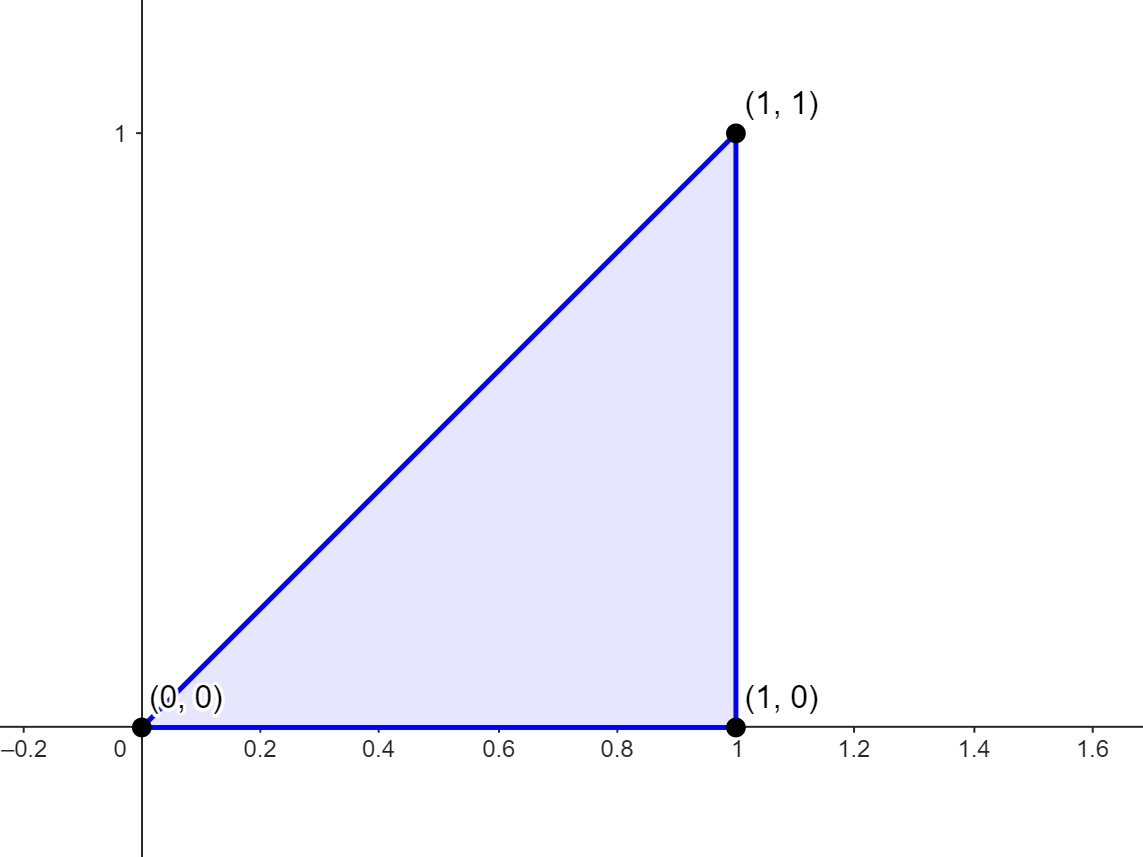
\includegraphics[width=\textwidth]{Capitoli/Capitolo4/Integrale 1.png}
    \end{minipage}
    \hfill
    \begin{minipage}{0.55\textwidth} 
    Tale insieme è un dominio normale sia rispetto all'asse $x$ che rispetto all'asse $y$. Si osservi che il risultato di tale integrale deve essere lo stesso in qualsiasi dei due casi.
    \end{minipage}
    \end{figure}
    Si consideri $D$ normale rispetto all'asse $x$, cioè:
    \begin{equation*}
        D= \left\{(x,y) \mid 0 \leq x \leq 1, 0 \leq y \leq x \right\}
    \end{equation*}
    Allora, applicando le formule di riduzione \eqref{Eq: Formula di riduzione integrali doppi 1}
    \begin{equation*}
    \begin{aligned}
        \iint\limits_D{xy}\,dx\,dy &= \int_{0}^{1}{\left(\int_{0}^{x}xy\,dy\right)}\,dx=  \int_{0}^{1}{x\left(\frac{y^2}{2}\Big|_{0}^{x}\right)\,dx = \int_{0}^{1}\frac{x^3}{2}\,dx} = \frac{1}{8}
    \end{aligned}
    \end{equation*}
    Considerando $D$ normale rispetto all'asse $y$
    \begin{equation*}
        D= \left\{(x,y) \mid 0 \leq y \leq 1, y \leq x \leq 1 \right\}
    \end{equation*}
    Allora applicando le formule di riduzione \eqref{Eq: Formula di riduzione integrali doppi 2}
    \begin{equation*}
        \iint\limits_D{xy}\,dx\,dy= \int_{0}^{1}{\left(\int_{y}^{1}{xy\,dx}\right)}\,dy = \int_{0}^{1}{y\left( \frac{x^2}{2}\Big|_{y}^1 \right)}\,dy= \frac{1}{2}\int_{0}^{1}{\left(y-y^3\right)}\,dy= \frac{1}{8}
    \end{equation*}
\end{example}
%\begin{example}[TO-DO]
%    Si consideri il seguente integrale doppio.
%    \begin{equation*}
%    \iint\limits_D e^\frac{x}{y}\, dx\,dy    
%    \end{equation*}
%    su $D=\left\{ (x,y) \mid \frac{1}{2} \leq x \leq 1, \sqrt[3]{x} \leq y \leq 1\right\}$
%\end{example}
\subsubsection{Formula di cambiamento di variabili}
Così come si faceva per gli integrali in una dimensione, anche per gli integrali in due dimensioni è possibile effettuare cambi di variabile. Prima di mostrare come sia possibile, occorre fare delle precisazioni a quanto detto in precedenza.
\begin{definition} \label{Def: Dominio regolare}
    Si dice che $D$ è un \textbf{dominio normale regolare} se, presi $a,b \in \mathbb{R}$ e $f,g, \in C^1([a,b])$ tali che $f < g\ \forall x \in (a,b)$ è della forma
    \begin{equation}
        D= \left\{a \leq x \leq b, \ f(x) \leq y \leq g(x) \right\}
    \end{equation}
    Si può anche dire che $D \subset \mathbb{R}$ è normale regolare se è un'unione finita di domini normali regolari che non abbiano punti interni in comune.
    \end{definition}
    %\begin{oss}
    %\end{oss}
    \vspace*{6pt}
Per poter approfondire il discorso occorre capire cosa si intenda per funzione con derivata prima continua su un chiuso. Si supponga dunque $f: \Omega \to \mathbb{R}$ con $\Omega = \overline{\mathring{\Omega}}$ e $f \in C^0(\Omega)$. Se $x_0 \in \mathring{\Omega}$ è noto il significato di derivate parziali continue in $x_0$. Al contrario, se $x_0 \in \partial \Omega$, si definiscono, se esistono:
\begin{equation}
\begin{aligned}
    &\frac{\partial{f}}{\partial{x}}(x_0)= \lim_{\substack{x \to x_0 \\ x \in \mathring{\Omega}}} \frac{\partial f}{\partial x}(x)\\
    &\frac{\partial{f}}{\partial{y}}(x_0)= \lim_{\substack{x \to x_0 \\ x \in \mathring{\Omega}}} \frac{\partial f}{\partial y}(x)
\end{aligned}
\end{equation}
dove si suppone $f \in C^1(\mathring{\Omega})$.\\
È necessario svolgere tale precisazione perché per effettuare il cambio di variabili occorre definire una funzione a valori vettoriali che abbia come dominio l'insieme di integrazione nelle nuove variabili e come codominio quello nelle variabili originali. Pertanto, si consideri ora una funzione a valori vettoriali definita su due domini regolari, $D,\ D' \subseteq \mathbb{R}^2$ della forma:
\begin{equation}
\begin{aligned}
    \Phi: D' &\to D\\
    (u,v) &\mapsto \Phi(u,v)
\end{aligned}
\end{equation}
con $\Phi(u,v)=(\Phi_1(u,v), \Phi_2(u,v))$ e $\Phi \in C^1(D')$, con le derivate parziali prolungate in $\partial D'$ come sopra. Allora su di essa può essere definita la Jacobiana 
\begin{equation}
    J_f(u,v)=\begin{pmatrix}
        \frac{\partial \Phi_1}{\partial x}(u,v) & \frac{\partial \Phi_1}{\partial y} (u,v)\\
        \frac{\partial \Phi_2}{\partial x} (u,v) & \frac{\partial \Phi_2}{\partial y} (u,v)
    \end{pmatrix}
\end{equation}
Ciò detto, si è in possesso di tutti gli strumenti necessari per la formulazione del teorema di cambiamento di variabili.
\begin{theorem}[Formula di cambiamento di variabili] \label{Teo: Formula cambiamento variabili}
    Siano $D, D'$ domini regolari di $\mathbb{R}^2$ e $\Phi: D' \to D$ di classe $C^1$ biunivoca e tale che $\det(J_f(u,v)) \neq 0\ \forall(u,v) \in D'$. Allora, per ogni $f \in C^0(D)$ vale
    \begin{equation} \label{Eq: Formula cambiamento di variabili}
        \iint\limits_{\substack{D\\=\Phi(D')}}
        f(x,y)\,dx\,dy= \iint\limits_{\substack{D'\\=\Phi^{-1}(D)}}{f(\Phi_1(u,v), \Phi_2(u,v))\left|\det(J_\Phi(u,v))\right|}\,du\,dv
    \end{equation}
\end{theorem}
\begin{example}
    Si risolva il seguente integrale.
    \begin{equation*}
        \iint\limits_{D}{\frac{x^3y}{x^2+y^2}\,dx\,dy}
    \end{equation*}
    con $D$ porzione di corona circolare con $r_1=1$ e $r_2=2$ nel primo quadrante compresa tra $y=\tfrac{\sqrt{3}}{3}x$ e $y=\sqrt{3}x$
\begin{figure}[H]
    \begin{minipage}{0.3\textwidth}
   \centering
   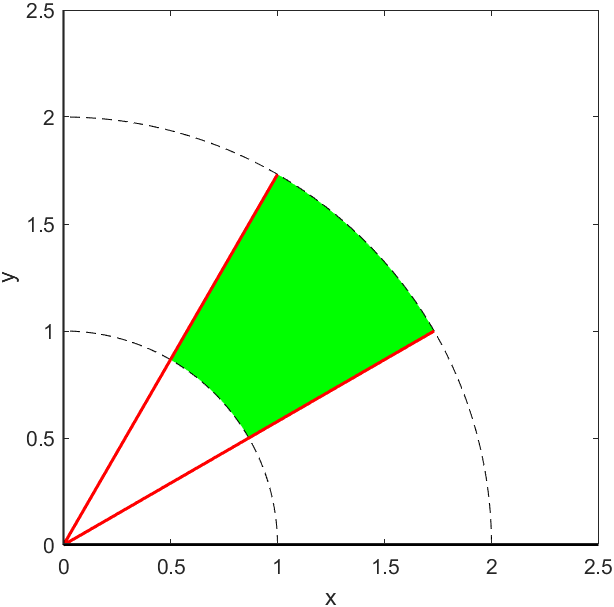
\includegraphics[width=\textwidth]{Capitoli/Capitolo4/Integrale 2.png}
    \end{minipage}
    \hfill
    \begin{minipage}{0.55\textwidth}
    In questo caso si può osservare come passando in coordinate polari sia estremamente più comodo risolvere tale integrale.\\
    Quindi
    \begin{equation*}
        \begin{cases}
            x= \varrho \cos \vartheta\\
            y= \varrho \sin \vartheta
        \end{cases}
    \end{equation*}
    Inoltre, lo Jacobiano è:
    \begin{equation*}
        \det\left(J_f(\varrho, \vartheta)\right)=\begin{vmatrix}
        \cos \vartheta & -\varrho \sin\vartheta\\
        \sin \vartheta & \varrho \cos\vartheta    
        \end{vmatrix}= \varrho
    \end{equation*}
    e $\arctan(\sqrt{3})= \tfrac{\pi}{3}$ e $\arctan(\tfrac{sqrt{3}}{3})=\tfrac{\pi}{6}$.
    \end{minipage}
\end{figure}
Pertanto, l'integrale diventa:
\begin{align*}
    &\iint\limits_{(\varrho, \vartheta) \in \Gamma=\left\{ 1 \leq \varrho \leq 2,\ \frac{\pi}{6} \leq \vartheta \frac{\pi}{3}\right\}}{\frac{\varrho^5 \cos^3 \vartheta \sin \vartheta}{\varrho^2}\,d\varrho\,d\vartheta}=\iint\limits_{\Gamma}{\varrho^3\left(\ \cos^3 \vartheta \sin \vartheta \right)\, d\varrho\,d\vartheta }=\\
    &=\int_{1}^{2}{\varrho^3\, d\varrho} \int_{\frac{\pi}{6}}^{\frac{\pi}{3}}{\cos^3\vartheta \sin \vartheta \, d\vartheta} = \left(\frac{\varrho^4}{4}\Big|_{1}^{2}\right)\left(\frac{\cos^4(\vartheta)}{4}\Big|_{\frac{\pi}{6}}^\frac{\pi}{3}\right)= \frac{15}{32}
    \end{align*}
\end{example}
Si presti attenzione a quanto segue. Nel caso descritto sopra, l'angolo $\vartheta$ era definito su $\left[\tfrac{\pi}{6}, \tfrac{\pi}{3}\right]$ e dunque non presentava problemi.\\
Tuttavia, per quanto affermato nelle ipotesi del teorema \ref{Teo: Formula cambiamento variabili}, è necessario che $\Phi$ sia biunivoca affinché il cambiamento sia ammesso. Dunque, non è altrettanto garantito il cambiamento di variabili se $\vartheta \in [0, 2\pi]$, poiché $\Phi(\varrho, 0)=\Phi(\varrho, 2\pi)$ ovvero $\Phi$ non è biunivoca.
Tuttavia, per ovviare a tale problema, è possibile estendere il teorema menzionato prima nella forma che segue.
\begin{theorem}
    Sia $\Phi \in C^1(D')$ e siano $D'$ e $\Phi(D')=D$ unioni finite di domini normali. Esista poi una successione di domini regolari $D'_k \subseteq D'$ tale che $\Phi\big|_{D'_k}$ verifichi le ipotesi del teorema \ref{Teo: Formula cambiamento variabili}. Se
    \begin{equation}
        m(D'_k) \to m(D') \qquad m(\Phi(D'_k)) \to m(\Phi(D'))
    \end{equation}
    allora si può dire lo stesso per $D$.
\end{theorem}
\vspace*{6pt}
\begin{oss}
    Si osservi che il passaggio a coordinate polari non è l'unico cambio di variabile degli integrali doppi.\\
    Generalmente, ogni qual volta vi sia la possibilità di semplificare $D$ rendendolo un dominio semplice rispetto ad una nuova variabile, è bene cambiare.\\ 
    Un esempio di nuove variabili può essere quello dato da un passaggio in \textit{coordinate ellittiche}
    \begin{equation}
        \begin{cases}
            x=\frac{\varrho}{a} \cos \vartheta\\
            y=\frac{\varrho}{b}\sin\vartheta
        \end{cases} \qquad a,b >0
    \end{equation}
\end{oss}
\section{Integrali tripli}
Si studino ora gli integrali tripli. Così come per gli integrali doppi, vale il discorso sulla costruzione mediante somme di Riemann. 
Si passi ora a descrivere le formule di riduzione.
\subsubsection{Formule di riduzione}
Siano $\mathcal{D}$ e $\mathcal{E}$ così definiti.
\begin{align}
    &\mathcal{D}=\left\{(x,y,z) \in \mathbb{R}^3 \mid (x,y) \in D \subseteq \mathbb{R}^2,\ \alpha(x, y)\leq z \leq \beta(x,y) \right\}\\
    &\mathcal{E}= \left\{(x,y,z) \in \mathbb{R}^3 \mid c_1\leq z \leq c_2, (x,y) \in D(z)\right\}
\end{align}
dove con $D$ si intende un dominio semplice. Siano poi $F \in C^0(\mathcal{D})$ e $G \in C^0(\mathcal{E}$.
Allora si dice che l'integrale è calcolato per \textit{fili paralleli} a $z$ se
\begin{equation}
    \iiint\limits_{\mathcal{D}} F(x,y,z)\, dx\, dy\,dz= \iint\limits_{D}{\left(\int_{\alpha(x,y)}^{\beta(x,y)}{F(x,y,z)\, dz}\right)}\,dx\, dy
\end{equation}
In alternativa, si dice che l'integrale è calcolato per \textit{strati paralleli} al piano $xy$ se
\begin{equation}
\iiint\limits_{\mathcal{E}}{G(x,y,z)\, dx\,dy\,dz} = \int_{c_1}^{c_2}{\left(\ \iint\limits_{D(z)}{G(x,y,z) \, dx\,dy} \right)\, dz}
\end{equation}
%\begin{example}[TO-DO]
%   Si calcoli il seguente integrale
%   \begin{equation*}
%\iiint\limits_{\mathcal{D}}{x^3z}\,dx\,dy\,dz
%   \end{equation*}
 %   su $\mathcal{D}= \left\{(x,y,z) \in \mathbb{R}^3 \mid z \geq 0,\ x^2+y^2+z^2\leq R^2\right\}$
%\end{example}
\begin{oss}    
Si noti che integrare (in due o tre dimensioni) sulla costante $1$ equivale a calcolare la misura dell'insieme di integrazione ovvero, nel primo caso, calcolarne l'area, nel secondo, il volume.
\end{oss}
\subsubsection{Formule di cambiamento di variabili}
Anche nel caso di integrali in $R^3$ si può pensare di effettuare dei cambi di variabile. Il teorema delle formule di cambiamento delle variabili in $\mathbb{R}^3$ è pressoché analogo a quello in due dimensioni e raggiunge la seguente tesi:
\begin{equation}
    \iiint\limits_{\mathcal{D}}{f(x,y,z)}\,dx\,dy\,dz=\iiint_{\mathcal{D}'}{f(u,v,w)|\det(J_\Phi)|}\,du\,dv\,dw
\end{equation}
Si mostrino alcuni cambi di variabili notevoli.

Siano dette $\varphi \in [0, \pi]$ latitudine, $\vartheta \in [0, 2\pi]$ longitudine e sia $\varrho \in [0, R]$ con $R$ raggio della sfera, allora si dicono \textit{coordinate sferiche}
\begin{equation}
    \begin{cases}
    x=\varrho \sin \varphi \cos \vartheta\\
    y=\varrho \sin \varphi \sin \vartheta\\
    z=\varrho \cos \varphi
    \end{cases}
\end{equation}
ed il modulo del determinante della Jacobiana ottenuta da questo cambio di parametri vale $\varrho^2 \sin \varphi$.\\
Si parla invece di \textit{coordinate cilindriche} quando si applica
\begin{equation}
    \begin{cases}
        x=\varrho \cos \varphi\\
        y=\varrho \sin \varphi\\
        z=w
    \end{cases}
\end{equation}
ed il modulo del determinante della Jacobiana vale $\varrho$.
\subsubsection{Volume di solidi di rotazione}
Un'applicazione dell'integrale di volume è il calcolo dei volumi dei solidi di rotazione, ovvero quei solidi ottenuti dalla rotazione del grafico $G(f)$ di una funzione $f:[a,b] \to \mathbb{R}^+$ tale che $z \mapsto y$ attorno all'asse $z$ di un angolo di $2\pi$. Nello specifico vale il teorema di Pappo-Guldino.
\begin{theorem}[Teorema di Pappo-Guldino]
Sia $\Omega$ un solido di rotazione ottenuto come detto sopra. Allora
\begin{equation}
    \text{Vol}(\Omega)= \pi \int_a^b{f(z)^2}\, dz
\end{equation}
\end{theorem}
\begin{proof}
    Si rappresenti $\Omega$ per strati paralleli a $xy$. Ogni strato è un cerchio della forma $x^2+y^2 \leq f(z)^2$ con $z$ fissato, $a<z<b$ per costruzione.
    Quindi, 
    \begin{equation}
    \begin{aligned}
        \text{Vol}(\Omega)&= \iiint\limits_{\Omega}\,dx\,dy\,dz=\int_a^b{\left(\iint\limits_{\{x^2+y^2 \leq f(z)^2\}}{\,dx\,dy}\right)}\,dz=\\
        &= \int_{a}^{b}{\text{Area}(x^2+y^2 \leq f(z)^2)}\,dz = \pi\int_a^b{f(z)^2}\,dz
    \end{aligned}
    \end{equation}
\end{proof}
\section{Integrali impropri}
Anche in $\mathbb{R}^n$ è possibile definire gli \textbf{integrali impropri} (o generalizzati). In tal caso, occorre distinguere due possibili casi più un terzo che generalizza.
\paragraph{$\mathbf{\Omega \subseteq \mathbb{R}^n}$ illimitato; $\mathbf{f \in C^0(\Omega)}$ positiva}
Si può dire che $\Omega$ è misurabile se, per ogni plurirettangolo $P$ di $\mathbb{R}^n$ limitato, $\Omega \cap P$ è misurabile. Allora supponendo $\Omega$ tale, si consideri una successione crescente di $\Omega$ misurabili e limitati tale che 
\begin{equation}
 \Omega_j<\Omega_{j+1}\ \forall j \qquad \bigcup\limits_{j}{\Omega_j}=\Omega
\end{equation}
Allora, poiché $f$ è integrabile su $I_j=\int\limits_{\Omega_j}{f}$, si dice che $f$ è \textbf{integrabile in senso improprio} se esiste finito
\begin{equation}
    \lim_{j \to +\infty} I_j := \int\limits_\Omega{f}\,dx_1\, \dots \,dx_n
\end{equation}
\paragraph{$\mathbf{\Omega \subseteq \mathbb{R}^n}$ limitato; $\mathbf{f \in C^0(\Omega)}$ illimitata e positiva} Come prima, si può trattare $\Omega$ come unione di insiemi $\Omega_j$ misurabili in cui la funzione sia limitata. Allora, se esiste finito, si definisce \textbf{integrale improprio} di $f$
\begin{equation}
    \lim_{j \to +\infty} \int\limits_{\Omega_j}f :=    \int\limits_{\Omega} f\,dx_1\, \dots \,dx_n
\end{equation}
\paragraph{$\mathbf{f, \Omega}$ come prima ma $\mathbf{f}$ cambia segno} In tal caso si considerano le funzioni parte positiva e parte negativa definite come:
\begin{equation}
    f^+(x)=\max\{f(x), 0\} \qquad f^-(x)=\min\{-f(x), 0\}
\end{equation}
e, se $f^+,\ f^-$ sono integrabili impropriamente, si definisce l'integrale improprio di $f$ come:
\begin{equation*}
    \int\limits_{\Omega}f := \int\limits_{\Omega} f^+ - \int\limits_{\Omega} f^-
\end{equation*}
\subsubsection{Integrale della Gaussiana}
Si mostri infine un'applicazione dell'integrale improprio.
\begin{theorem}[Integrale della Gaussiana]
    \begin{equation}
    \int_{-\infty}^{+\infty}{e^{-x^2}}\, dx = \sqrt{\pi}
    \end{equation}
\end{theorem}
\begin{proof}
    Si consideri innanzitutto il seguente integrale
    \begin{equation}
        I=\iint\limits_{\mathbb{R}^2}{e^{-(x^2+y^2)}}\,dx\,dy
    \end{equation}
    Per quanto detto, se tale integrale esiste allora può essere calcolato come
    \begin{equation} \label{Eq: Primo risultato teorema integrale gaussiana}
    \begin{aligned}
        I&=\lim_{R \to +\infty}{\iint_{B_R(0)}{e^{-(x^2+y^2)}}}\,dx\,dy \overset{\text{Polari}}{=} \lim_{R \to +\infty}{\iint\limits_{\substack{0 \leq \varrho \leq R^2\\ 0 \leq \vartheta \leq 2\pi}}{e^{-\varrho^2} \varrho}\,d\varrho\,d\vartheta}=\\
        &= 2\pi \lim_{R \to +\infty}{\frac{1}{2}}{\left( -e^{-\varrho^2}\right) \Big|_{0}^{R}}= \pi \lim_{R \to +\infty}{(1-e^{-R^2})}= \pi
    \end{aligned}
    \end{equation}
    Tuttavia, la partizione tramite palle di raggio $R$ non è l'unica possibile. Si suddivida $\mathbb{R}^2$ in quadrati della forma
    \begin{equation}
        Q_j=(-J,J) \times (-J, J)
    \end{equation}
    Allora, 
    \begin{equation}
    \begin{aligned}
        I&= \lim_{J \to +\infty}{\iint\limits_{Q_J}{e^{-(x^2+y^2)}}\,dx\,dy}\overset{\eqref{Eq: Integrale doppio di funzioni separate}}{=} \lim_{J \to +\infty}{\int_{-J}^{+J}{e^{-x^2}}\, dx\ \int_{-J}^{+J}{e^{-y^2}}\,dy}=\\
        &=\lim_{J \to + \infty}\left(\int_{-J}^{+J}{ e^{-x^2}}\,dx\right)^2 = \left(\int_{-\infty}^{+\infty}{ e^{-x^2}}\,dx\right)^2 \overset{\eqref{Eq: Primo risultato teorema integrale gaussiana}}{=} \pi
    \end{aligned}
    \end{equation}
    Ne consegue che
    \begin{equation}
        \int_{-\infty}^{+\infty}{e^{-x^2}}\, dx = \sqrt{\pi}
    \end{equation}
\end{proof}